\documentclass{article}
\usepackage[T2A]{fontenc}
\usepackage[utf8]{inputenc}
\usepackage[a4paper,
            mag=1000, includefoot,
            left=3cm, right=1.5cm, top=2cm, bottom=2cm, headsep=1cm, footskip=1cm]{geometry}

\usepackage[english,russian]{babel}
\usepackage{indentfirst}
\usepackage{amsfonts}
\usepackage{amsmath}
\usepackage{amsthm}
\usepackage{bbold}
\usepackage{moreverb}
\usepackage{dsfont}
\usepackage{graphicx}
\usepackage{bm}
\usepackage{booktabs} 


\usepackage[colorlinks=true]{hyperref}

\DeclareMathOperator{\tr}{tr}
\DeclareMathOperator*{\argmin}{arg\,min}
\DeclareMathOperator*{\argmax}{arg\,max}
\DeclareMathOperator{\sign}{sign}
\DeclareMathSymbol{\intercal}     {\mathbin}{AMSa}{"7C}
\newtheorem{theorem}{Теорема}
\newtheorem{task}{Задача}


\title{Обучение с учителем. Классификация. Дискриминантный анализ. Логистическая регрессия. Метод опорных векторов. Выбор модели с помощью кросс-валидации. Метод стохастического градиента.}
\author{Белкова Анна, Редкокош Кирилл, Лобанова Полина, гр. 21.M03-мм}
\date{\today}

\begin{document}
	\maketitle
	\tableofcontents
	\newpage
	
	\section{Классификация}
	\subsection{Постановка задачи}

Дано:
    \begin{itemize}
        \item X -- матрица признаков, где $\boldsymbol{x}_i \in \mathbb{R}^p$ -- $i$ вектор этой матрицы (признаки $i$ индивида).
        \item $\mathcal{Y}$ -- конечное множество номеров (имён, меток) классов, где  $y_i \in \mathcal{Y}$, a $\boldsymbol{y}$ --- вектор меток классов для матрицы X.
    \end{itemize}

Задача:
\begin{itemize}

\item По выборке $(X_{train},\boldsymbol{y}_{train})$, построить классификатор $f:\mathbb{R}^p\to \mathcal{Y}$, который по выборке $(X_{test},\boldsymbol{y}_{test})$ предскажет метку класса.

       \item Хотим, чтобы на $f$ достигается минимальная ошибка классификации в некотором смысле.
\end{itemize} 

На генеральном языке:
    \begin{itemize}
        \item $\boldsymbol{\xi}\in\mathbb{R}^p$ -- случайный вектор признаков.
        \item $\eta\in\mathcal{Y}$ -- дискретная случайная величина, метка класса.
        \item $P(\boldsymbol{\xi},\eta)$ -- их совместное распределение.
    \end{itemize}
    
Дано:

Выборка $(X_{train},\boldsymbol{y}_{train})$ -- $N$ реализаций случайного вектора $(\boldsymbol{\xi},\eta)$, по выборке необходимо построить классификатор $$f:\mathbb{R}^p\to \mathcal{Y}.$$


Линейная модель классификации в общем случае:
$f(\boldsymbol{x}_i,\boldsymbol{w})=sign\langle\boldsymbol{w},\boldsymbol{x}_i\rangle$, где $\boldsymbol{w}$ вектор весов признаков, а $w_0$ некоторый сдвиг, который позволяет нам не получить 0 значение.


Мы будем рассматривать классификатор в следующей форме, добавив вектор из единиц:
$$f(\boldsymbol{x}_i,\boldsymbol{w})=sign\langle\boldsymbol{w},\boldsymbol{x}_i\rangle.$$

Отступ (margin): $M_i=\langle (\boldsymbol{w}, \boldsymbol{x}_i),\boldsymbol{x}_i\rangle y_i$ ---  "расстояние" между реальным и предсказанным значением . В случае отрицательного значения, считаем, что объект не принадлежит классу. 

Функцию потерь $\mathcal{L}(M)$--- неотрицательная функция, характеризующая величину ошибки предсказания. Пороговая функция потерь: $[M(x_i)<0]$.

Тогда задача классификации можно свести к минимизации функции потерь:
$$\mathcal{L}(M)\to \min$$

Далее будем рассматривать отступ,  со знаком минус, как штраф за неверную классификацию.


\begin{figure}[h!]
\center{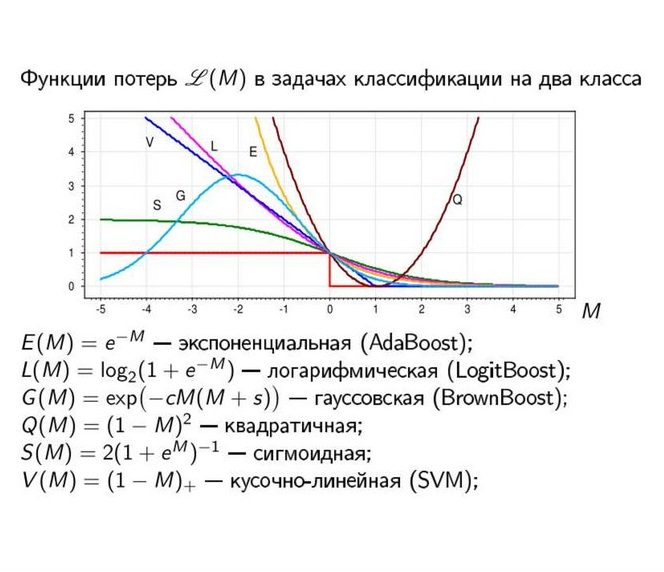
\includegraphics[scale=0.95]{slide-7.jpg}}
\end{figure}

	\subsection{Метрики качества классификации}
	Часто возникает необходимость в изучении различных аспектов качества уже обученного классификатора.
	Обсудим подробнее распространённые подходы к измерению качества моделей.
	\subsubsection{Матрица ошибок}
	
	Перед переходом к самим метрикам необходимо ввести важную концепцию для описания этих метрик в терминах ошибок классификации — confusion matrix (матрица ошибок).
	
	Допустим, что у нас есть два класса и алгоритм, предсказывающий принадлежность каждого объекта одному из классов, тогда матрица ошибок классификации будет выглядеть следующим образом:
	
	\begin{table}[hhh]
		\begin{tabular}{|l|l|l|}
			\hline
			& y=1                 & y=0                 \\ \hline
			$\hat y = 1$ & True Positive (TP)  & False Positive (FP) \\ \hline
			$\hat y = 0$ & False Negative (FN) & True Negative (TN) \\ \hline
		\end{tabular}
	\end{table}

	Где $\hat y$ — это ответ алгоритма на объекте, а $y$ — истинная метка класса на этом объекте.
	Таким образом, ошибки классификации бывают двух видов: False Negative (FN) и False Positive (FP).
	
	\subsubsection{Accuracy}
	
	Интуитивно понятной, очевидной и почти неиспользуемой метрикой является accuracy — доля правильных ответов алгоритма:
	
	\begin{align*}
	accuracy = \frac{TP + TN}{TP + TN + FP + FN}
	\end{align*}
	
	Эта метрика бесполезна в задачах с неравными классами, и это легко показать на примере.
	
	Допустим, мы хотим оценить работу спам-фильтра почты. У нас есть 100 не-спам писем, 90 из которых наш классификатор определил верно (True Negative = 90, False Positive = 10), и 10 спам-писем, 5 из которых классификатор также определил верно (True Positive = 5, False Negative = 5).
	Тогда accuracy:
	
	\begin{align*}
		accuracy = \frac{5 + 90}{5 + 90 + 10 + 5} = 86,4\% 
	\end{align*}
	
	Однако если мы просто будем предсказывать все письма как не-спам, то получим более высокую accuracy:
	
	\begin{align*}
		accuracy = \frac{0 + 100}{0 + 100 + 0 + 10} = 90,9\% 
	\end{align*}
	
	При этом, наша модель совершенно не обладает никакой предсказательной силой, так как изначально мы хотели определять письма со спамом. Преодолеть это нам поможет переход с общей для всех классов метрики к отдельным показателям качества классов.
	
	\subsubsection{Precision, recall и F-мера}
	
	Для оценки качества работы алгоритма на каждом из классов по отдельности введем метрики precision (точность) и recall (полнота).
	
	\begin{align*}
	precision = \frac{TP}{TP + FP}
	\end{align*}

	\begin{align*}
	recall = \frac{TP}{TP + FN}
	\end{align*}
	
	Precision можно интерпретировать как долю объектов, названных классификатором положительными и при этом действительно являющимися положительными, а recall показывает, какую долю объектов положительного класса из всех объектов положительного класса нашел алгоритм.
	
	Именно введение precision не позволяет нам записывать все объекты в один класс, так как в этом случае мы получаем рост уровня False Positive. Recall демонстрирует способность алгоритма обнаруживать данный класс вообще, а precision — способность отличать этот класс от других классов.
	
	Precision и recall не зависят, в отличие от accuracy, от соотношения классов и потому применимы в условиях несбалансированных выборок.
	
	Существует несколько различных способов объединить precision и recall в агрегированный критерий качества. F-мера (в общем случае $\ F_\beta$) — среднее гармоническое precision и recall :
	
	\begin{align*}
	\ F_\beta = (1 + \beta^2) \cdot \frac{precision \cdot recall}{(\beta^2 \cdot precision) + recall}
	\end{align*}
	
	$\beta$ в данном случае определяет вес точности в метрике, и при $\beta = 1$ это среднее гармоническое (с множителем 2, чтобы в случае precision = 1 и recall = 1 иметь $\ F_1 = 1$)
	F-мера достигает максимума при полноте и точности, равными единице, и близка к нулю, если один из аргументов близок к нулю.
	
	\subsubsection{AUC-ROC и AUC-PR}
	
	Одним из способов оценить модель, является AUC-ROC (или ROC AUC) — площадь (Area Under Curve) под кривой ошибок (Receiver Operating Characteristic curve ). Данная кривая представляет из себя линию от (0,0) до (1,1) в координатах True Positive Rate (TPR) и False Positive Rate (FPR):
	
	\begin{align*}
		TPR = \frac{TP}{TP + FN}
	\end{align*}	
	
	\begin{align*}
		FPR = \frac{FP}{FP + TN}
	\end{align*}

	TPR-- это полнота, а FPR показывает, какую долю из объектов negative класса алгоритм предсказал неверно. В идеальном случае, когда классификатор не делает ошибок (FPR = 0, TPR = 1) мы получим площадь под кривой, равную единице; в противном случае, когда классификатор случайно выдает вероятности классов, AUC-ROC будет стремиться к 0.5, так как классификатор будет выдавать одинаковое количество TP и FP.
	
	\begin{figure}[hhh!]
		\begin{center}
			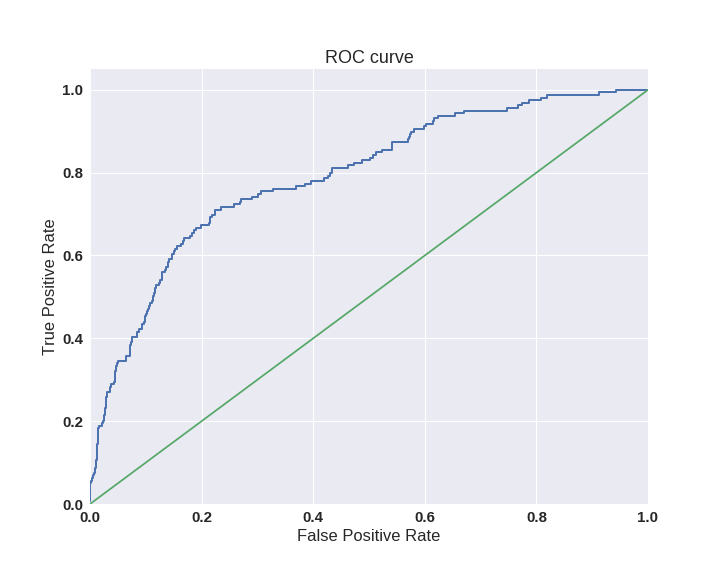
\includegraphics[width=12cm]{299157fad56a4ecca8f6b96b425bd38c}
		\end{center}
		\vspace{-5mm}\caption{ROC-кривая}
	\end{figure}
	
	Каждая точка на графике соответствует выбору некоторого порога. Площадь под кривой в данном случае показывает качество алгоритма.
	
	Precision и recall также используют для построения кривой и, аналогично AUC-ROC, находят площадь под ней:
	
	\begin{figure}[hhh!]
		\begin{center}
			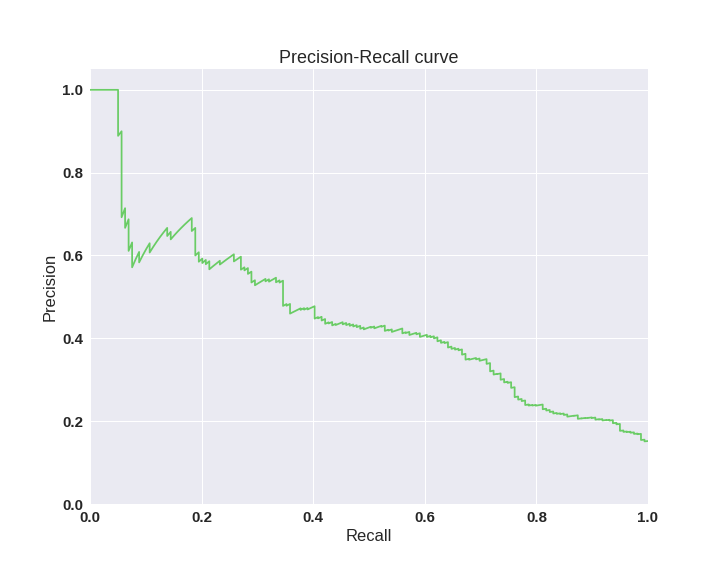
\includegraphics[width=12cm]{8873569147c24b49a2b7fa9ae883f20f}
		\end{center}
		\vspace{-5mm}\caption{PR-кривая}
	\end{figure}
	
	\subsection{Модификации датасета для выравнивания соотношения классов}
	
	Одним из распространенных способов решения проблемы несбалансированных данных является избыточная выборка. Чрезмерная выборка относится к различным методам, которые направлены на увеличение количества экземпляров из недопредставленного класса в наборе данных.
	
	\subsubsection{Случайная наивная избыточная выборка}
	
	Самый простой способ сделать это - случайным образом выбрать наблюдения из класса меньшинства и добавить их в набор данных, пока мы не достигнем баланса между большинством и классом меньшинства. 
	
	Одна проблема со случайной наивной избыточной выборкой заключается в том, что она просто дублирует уже существующие данные. Поэтому, хотя алгоритмы классификации подвергаются большему количеству наблюдений из класса меньшинства, они не узнают больше о том, как отличить наблюдения одного класса от другого. Новые данные не содержат больше информации о характеристиках класса, чем старые данные.
	
	\subsubsection{SMOTE}
	
	Метод увеличения числа примеров миноритарного класса (Synthetic Minority Over-sampling Technique, SMOTE) — это алгоритм предварительной обработки данных, используемый для устранения дисбаланса классов в наборе данных.
	
	В общих чертах этот алгоритм можно описать следующим образом.
	Он находит разность между данным образцом и его ближайшим соседом.
	Эта разность умножается на случайное число в интервале от 0 до 1.
	Полученное значение добавляется к данному образцу для формирования нового синтезированного образца в пространстве признаков.
	Подобные действия продолжаются со следующим ближайшим соседом, до заданного пользователем количества образцов.
	
	Проиллюстрируем алгоритм более подробно. Предположим, у нас есть несбалансированный набор данных (индивидов одного класса гораздо больше, чем другого).
	
	Берем индивида и вычисляем k-ближайших соседей. Затем выбираем случайного ближайшего соседа из k-ближайших соседей.
	
	\begin{figure}[hhh!]
		\begin{center}
			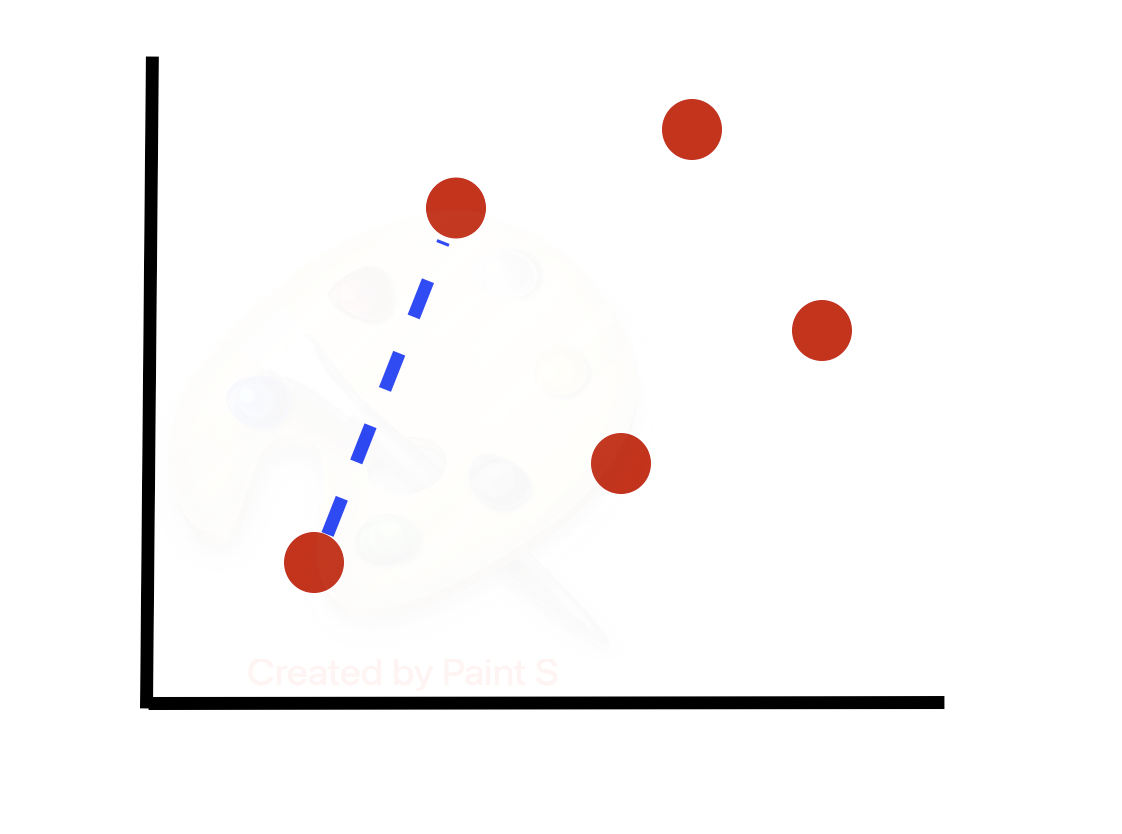
\includegraphics[width=10cm]{11.png}
		\end{center}
		\vspace{-5mm}
	\end{figure}

	Вычисляем разность между двумя точками и умножаем ее на случайное число от 0 до 1. Получаем синтезированный образец вдоль линии между двумя точками.
	
	\begin{figure}[hhh!]
		\begin{center}
			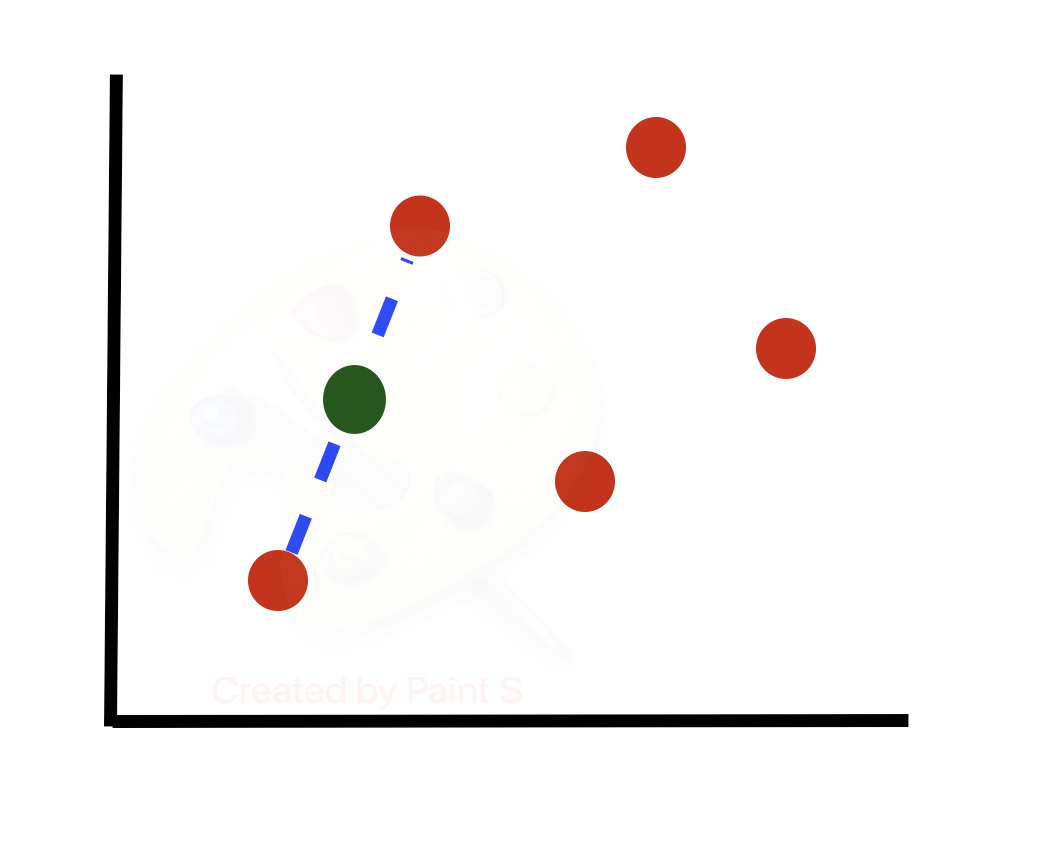
\includegraphics[width=10cm]{12.png}
		\end{center}
		\vspace{-5mm}
	\end{figure}

	Выбираем $m$ соседей для этого индивида и повторяем процедуру дублирования. $m$ подбирается из соотношения классов. 
	
	\begin{figure}[h!]
		\begin{center}
			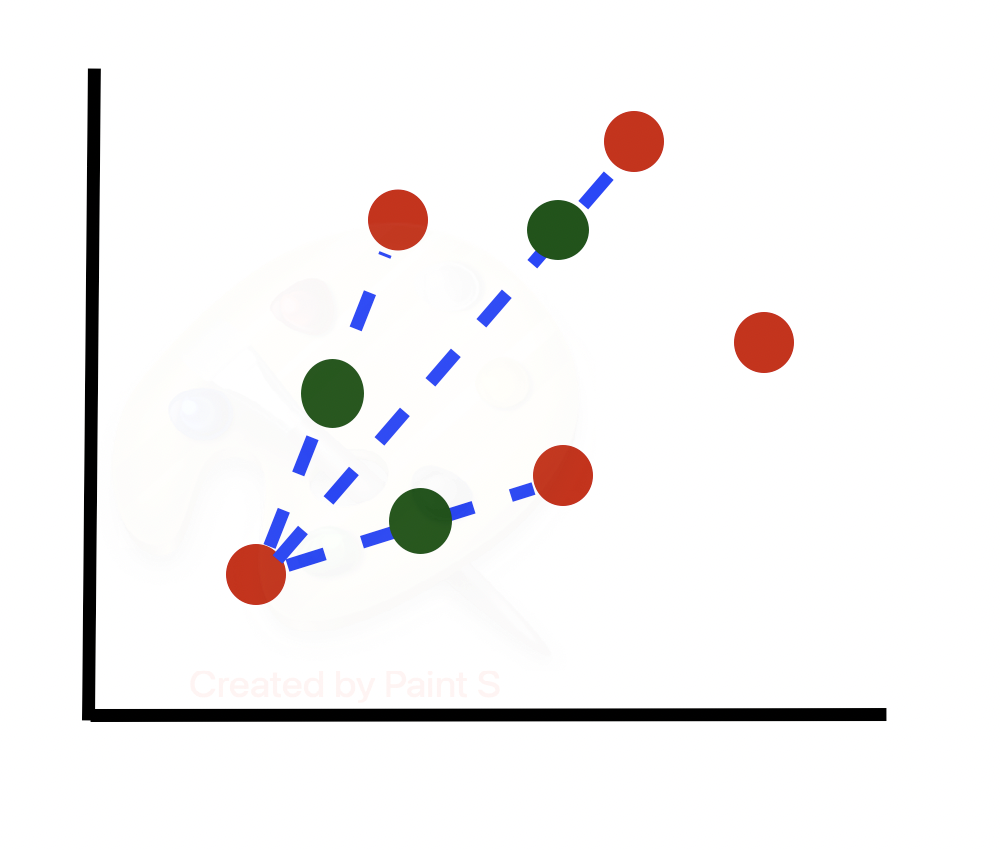
\includegraphics[width=10cm]{0_XvMdqBNsrjU5f8V5.png}
		\end{center}
		\vspace{-5mm}
	\end{figure}

	Для каждого из исходных индивидов повторяем весь алгоритм для достижения равного количества индивидов в классах.
	
	$\textbf{SMOTE Расширения}$
	
	Как и в большинстве алгоритмов, есть несколько расширений SMOTE. Они нацелены на улучшение SMOTE путем добавления его функциональности или уменьшения его слабых сторон. Примеры расширений SMOTE, которые можно найти в imblearn, включают:
	
	\begin{itemize}
		\item BorderlineSMOTE: Вместо избыточной выборки между всеми наблюдениями меньшинств, BorderlineSMOTE стремится увеличить количество наблюдений меньшинств, которые граничат с наблюдениями большинства. Цель здесь - дать классификатору возможность более четко различать эти пограничные наблюдения.
		\item SVMSMOTE: SVMSMOTE, как следует из его названия, использует алгоритм машины опорных векторов для генерации новых наблюдений меньшинства вблизи границы между классами большинства и меньшинства.
	\end{itemize}
	
	\subsubsection{Tomek Links}
	
	Пусть индивиды $E_i$ и $E_j$ принадлежат к различным классам, $d(E_i,E_j)$
	– расстояние между указанными примерами. Пара $(E_i,E_j)$
	называется связью Томека, если не найдется ни одного примера $E_l$
	такого, что будет справедлива совокупность неравенств:
	
	\begin{equation*}
		\begin{cases}
			d(E_i,E_l)<d(E_i,E_j),\\
			d(E_j,E_l)<d(E_i,E_j)
		\end{cases}
	\end{equation*}
	
	Согласно данному подходу, все индивиды из большей группы, входящие в связи Томека, должны быть удалены из набора данных. Этот способ хорошо удаляет записи, которые можно рассматривать в качестве «зашумляющих». Далее
	визуально показан набор данных в двумерном пространстве признаков до и после применения поиска связей Томека.
	
	\begin{figure}[hhh!]
		\begin{center}
			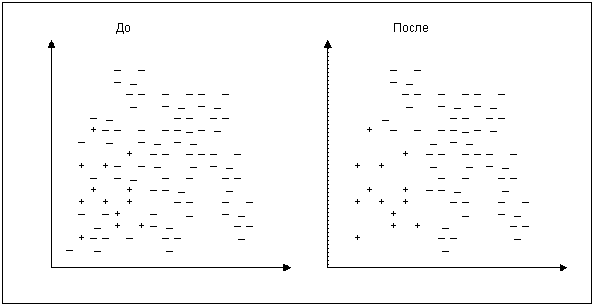
\includegraphics[width=10cm]{Tomek_links}
		\end{center}
		\vspace{-5mm}
	\end{figure}
	
	\section{Дискриминантный анализ}
	
	Суть дискриминантного анализа заключается в том, чтобы смоделировать распределение $X$ в каждом из классов отдельно, а затем использовать теорему Байеса, чтобы получить $P(Y = i \mid X = x)$ 
	
	\subsection{Байесовский классификатор}
	
	В качестве меры ошибки предсказания введем функцию потерь. Рассмотрим матрицу $\mathbf{L}$ размера $K \times K$, где $K = card(\mathcal{Y})$. На диагонали $\mathbf{L}$ стоят нули, а $\mathbf{L}(i,j) = \lambda_{ij}$ -- цена ошибки отнесения элемента класса $Y_i$ к классу $Y_j$. Часто используется 0-1 функция потерь, где каждая ошибка оценивается единицей.
	
	Математическое ожидание функции потерь (средний риск):
	\begin{align*}
		R(a) = \mathds{E}(\mathbf{L}(\eta, a(\xi))) = \mathds{E}_{\xi} \sum_{k = 1}^{K} L(Y_i, a(\xi)) P(Y_i \mid \xi).
	\end{align*}
	
	Отсюда получаем функцию классификации:
	\begin{align*}
		f(x) = \argmin_{Y \in \mathcal{Y}} \sum_{k = 1}^{K} L(Y_i, Y) P(Y_i \mid  \xi = x).
	\end{align*}
	Если подставим сюда 0-1 функцию потерь, получим
	\begin{align*}
		f(x) = \argmin_{Y \in \mathcal{Y}} 1 - P(Y \mid \xi = x).
	\end{align*}
	Или, что то же самое
	\begin{align*}
		f(x) = \argmax_{Y \in \mathcal{Y}} P(Y \mid \xi = x) = \argmax_{Y \in \mathcal{Y}} P(Y)P(\xi \mid \eta = Y).
	\end{align*}
	Это решение называется байесовским классификатором, а такой подход -- принципом максимума апостериорной вероятности.
	
	Для построения байесовского классификатора, нам необходимо знать апостериорные вероятности $P(Y \mid \xi = x)$.
	
	Обозначим $p_i(x) = P(\xi = x \mid \eta =Y_i)$ условные плотности классов, $\pi_i = P(\eta = Y_i)$ -- априорные вероятности, $\sum_{i = 1}^{K} \pi_i = 1$. По теореме Байеса получим:
	\begin{align*}
		P(Y = i \mid X = x) = \frac{p_i(x) \pi_i}{\sum_{i = 1}^K p_i(x)\pi_i}.
	\end{align*}
	
	Поэтому в качестве классифицирующих функций берут
	$$f_i\left(x\right) = \frac{p_i(x) \pi_i}{\sum_{j=1}^k p_j(x) \pi_j}. $$
	
	Так как знаменатель у всех $f_i$ одинаковый, его можно отбросить, и итоговые классифицирующие функции будут выглядеть как $f_i\left(x\right) = \mathrm P\left(x\middle\vert C_i\right) \pi_i = p_i(x) \pi_i$.
	
	Возникает вопрос: откуда брать априорные вероятности?
	\begin{enumerate}
		\item Равномерно, $\forall i \in 1\mathbin : k \; \pi_i = 1 \mathbin / k$.
		\item По соотношениям в обучающей выборке: $\pi_i = n_i \mathbin / \sum_{j=1}^k n_j$.
		\item На основе другой дополнительной информации о данных (результаты предыдущих исследований, etc.)
	\end{enumerate}

	Построенный метод классификации $\mathrm{predict}(x) = \argmax_i \pi_i p_i(x)$ минимизирует среднюю апостериорную ошибку:
	$$\sum_{i=1}^k \pi_i \mathrm P(\mathrm{predict}(x) != i\mid Y_i).$$
	
	\subsection{Линейный дискриминантный анализ}
	
	Модель: $\xi$ --- дискретная с.в., принимающая значения $\left\lbrace Y_i\right\rbrace_{i=1}^k$, $\mathcal P(\eta\mid \xi = Y_i) = \mathcal N (\mu_i, \mathbf\Sigma)$.  (Предполагаем, что классы имеют нормальное распределение с одинаковой ковариационной матрицей)
	
	Тогда плотность в точке $x$:
	
	$$p_i(x) = p\left(x\middle\vert \xi = Y_i\right) = \frac{1}{\left(2\pi\right)^{p/2}\left\vert\bm{\Sigma}\right\vert^{1/2}} \exp\left(-\frac{1}{2}{\left(x^T -\mu_i\right)}\bm{\Sigma}^{-1}\left(x -\mu_i\right)\right),$$
	
	и классифицирующая функция $f_i\left(x\right) = \pi_i p\left(x\middle\vert \xi = Y_i\right)$, где $\pi_i$ --- априорная вероятность наблюдения попасть в $i$-ю группу. Для упрощения вычислений можно переписать классифицирующую функцию через возрастающее монотонное преобразование как
	
	$$g_i\left(x\right) = \log f_i\left(x\right) = \log \pi_i - \frac{1}{2}\log\left\vert\bm{\Sigma}\right\vert -  \frac{1}{2}{\left(x^T -\mu_i\right)}\bm{\Sigma}^{-1}\left(x -\mu_i\right).$$
	Сократив часть, не зависящую от номера класса, получаем линейные классифицирующие функции:
	$$h_i(x) = -\frac{1}{2}{\mu_i}^T\bm{\Sigma}^{-1}\mu_i + {\mu_i}^T\bm{\Sigma}^{-1}x + \log\pi_i.$$
	
	\subsection{Канонические переменные}
	
	Задача: найти линейное преобразование $\mathbf{Z} = A^\mathrm{T}\mathbf{X}$, в результате которого получаются признаки наилучшим образом разделяющие группы.  Хотелось бы, чтобы эти признаки оказались ортогональны. Далее опишем эту задачу более формально.
	
	Вычислим внутриклассовую ковариационную матрицу:
		\begin{align*}
			\mathbf{E} = \frac{1}{n - K} \sum\limits_{i = 1}^K \sum_{j: y_j = Y_i} (x_j - \widehat{\mu}_i)^\mathrm{T}(x_j - \widehat{\mu}_i)
		\end{align*}
		Вычисляем межклассовую ковариационную матрицу (с точностью до коэффициента):
		\begin{align*}
			\mathbf{H} = \sum\limits_{i = 1}^K n_i (\widehat{\mu}_i - \widehat{\mu})^\mathrm{T}(\widehat{\mu}_i - \widehat{\mu}).
		\end{align*}
	
	Пусть $\zeta = A\xi$ -- новый признак, тогда распределение $P(\zeta \mid \eta = Y_k) = \mathcal{N}_p(A^\mathrm{T}\mu_k, A^\mathrm{T}\mathbf{\Sigma}_kA)$.
	
	На выборочном языке новые признаки $\mathbf{Z} =A^\mathrm{T}\mathbf{X}$. Выборочная ковариационная матрица (с точностью до коэффициента) новых признаков имеет вид:
	\begin{align*}
		A^\mathrm{T}\mathbf{T}A = A^\mathrm{T}(\mathbf{E} + \mathbf{H})A = A^\mathrm{T}\mathbf{E}A + A^\mathrm{T}\mathbf{H}A,
	\end{align*}
	где $\mathbf{T}$ -- total covariance matrix, первое слагаемое -- оценка внутригрупповых отклонений, а второе -- оценка межгрупповых отклонений. Воспользовавшись критерием Фишера перейдем к обобщенной задаче на собственные числа и собственные вектора:
	\begin{align*}
		\frac{A^\mathrm{T}\mathbf{H}A}{A^\mathrm{T}\mathbf{E}A} \rightarrow \max_{A}.
	\end{align*}
	
	Пусть $\lambda_1 \geq \lambda_2 \geq \ldots \geq \lambda_d$ -- собственные числа матрицы $\mathbf{E}^{-1}\mathbf{H}$, а $A_1, \ldots, A_d$ -- соответствующие им собственные вектора. Тогда максимум выше равен $\lambda_1$  и достигается на $A_1$. При этом $A^\mathrm{T}_i \mathbf{E}A_j = 0$. Далее
	\begin{align*}
		\max_{A, A \bot A_1}\frac{A^\mathrm{T}\mathbf{H}A}{A^\mathrm{T}\mathbf{E}A} = \lambda_2,
	\end{align*}
	достигается на $A_2$ и так далее.
	
	Вектора $A_i$ называют каноническими коэффициентами, а новые признаки $Z_i$ -- каноническими переменными, $Z_i$ ортогональны.
	
	\subsection{Значимость канонических переменных}
	
	Возникает вопрос: сколько канонических переменных нам окажется достаточно взять? Другими словами, нужно проверить гипотезу:
	
	\begin{align*}
		H_0: A_i, i = \ell,\ldots,d~\text{не описывают отличия}.
	\end{align*}
	Введем статистику $\Lambda-prime$ (Wilks' Lambda):
	\begin{align*}
		\Lambda_\ell^p = \prod_{i = l}^d \frac{1}{1 + \lambda_i}.
	\end{align*}
	Тогда гипотезу выше можно переформулировать так
	\begin{align*}
		H_0: \Lambda_\ell^p = 1 \Leftrightarrow \lambda_\ell = \ldots = \lambda_d = 0 \Leftrightarrow rank \mathbf{B} = \ell - 1.
	\end{align*}
	
	Критерий:
	\begin{align*}
		t = \Lambda_{\ell}^{p} \sim \Lambda_{\nu_\mathbf{B} + (\ell - 1), \nu_\mathbf{W} - (\ell - 1)}.
	\end{align*}
	
	Другими вариантами статистиками для проверки гипотезы могут являться:
	\begin{itemize}
	\item Roy's greatest root $$r_1^2 = \frac{\lambda_1}{1+\lambda_1};$$
	
	\item Pillai's trace $$V=trace(\mathbf H(\mathbf H + \mathbf E)^{-1});$$
	
	\item Hotelling-Lawley trace $$V=trace(\mathbf H \mathbf E^{-1}).$$
	\end{itemize}
	
	\subsection{Квадратичный дискриминантный анализ}
	
	Модель: $\xi$ --- дискретная с.в., принимающая значения $\left\lbrace Y_i\right\rbrace_{i=1}^k$, $\mathcal P(\eta\mid \xi = Y_i) = \mathcal N\left(\mu_i, \bm{\Sigma}_i\right)$. (Предполагаем, что каждый класс имеет многомерное нормальное распределение с различными ковариационными матрицами)
	
	Тогда плотность в точке $x$:
	$$p\left(x\middle\vert \xi = Y_i\right) = \frac{1}{\left(2\pi\right)^{p/2}\left\vert\bm{\Sigma}_i\right\vert^{1/2}} \exp\left(-\frac{1}{2}{\left(x^T -\mu_i\right)}\bm{\Sigma}_i^{-1}\left(x -\mu_i\right)\right),$$
	и классифицирующая функция $f_i\left(x\right) = \pi_i p\left(x\middle\vert \xi = Y_i\right)$. Применяем возрастающее монотонное преобразование и оставляем в классифицирующей функции только члены, отличающиеся в разных группах:
	
	$$g_i\left(x\right) = \log f_i\left(x\right) = \log \pi_i - \frac{1}{2}\log\left\vert\bm{\Sigma}_i\right\vert -  \frac{1}{2}{\left(x^T -\mu_i\right)}\bm{\Sigma}_i^{-1}\left(x -\mu_i\right),$$
	получаем квадратично зависящую от $x$ классифицирующую функцию.
	
	\subsection{Оценка параметров}
	На практике параметры распределений классов нам не известны, поэтому предлагается использовать следующие оценки максимального правдоподобия параметров нормальных плотностей классов.
	\begin{itemize}
		\item Среднее
		$\overline{\mu}_i = \frac{1}{n_i}\sum\limits_{j: y_j = Y_i} x_j$,
		\item Ковариационная матрица класса $\widehat{\mathbf{\Sigma}}_i = \frac{1}{n_i - 1}\sum\limits_{j: y_j = Y_i} (x_j - \overline{\mu}_i)^\mathrm{T}(x_j - \overline{\mu}_i)$,
		\item Pooled ковариационная матрица $\widehat{\mathbf{\Sigma}}= \sum\limits_{j = 1}^K\frac{n_i - 1}{n - K} \widehat{\mathbf{\Sigma}}_i$.
	\end{itemize}
	
	\subsection{Regularized Discriminant Analysis}
	Оценка ковариационной матрицы $\widehat{\mathbf{\Sigma}}_i$ может оказаться выражденной или плохо обусловленной. Опишем компромис между LDA и QDA, а так же борьбу с мультиколлинеарностью.
	\begin{itemize}
		\item Regularized Discriminant Analysis. Рассматривается матрица $\widehat{\mathbf{\Sigma}}_i(\alpha) = \alpha \widehat{\mathbf{\Sigma}}_i + (1 - \alpha)\widehat{\mathbf{\Sigma}}$, где $\widehat{\mathbf{\Sigma}}$ -- pooled ковариационая матрица. Здесь $\alpha \in [0, 1]$ порождает континуум моделей между LDA и QDA, выбирается скользящим контролем.
		\item Дополнительно к предыдущему методу можно похожим образом модифицировать pooled ковариационную матрицу и рассматривать $\widehat{\Sigma}(\gamma) = \gamma \widehat{\mathbf{\Sigma}} + (1 - \gamma)\sigma^2 \mathbf{I}_p$, где $\gamma$ определяет вид ковариационной матрицы и выбирается скользящим контролем.
	\end{itemize}
	
	\subsection{Наивный байесовский классификатор}
	Предположим, что признаки независимы внутри групп и имеют нормальное распределение:
	\begin{align*}
		p_i(x) = \prod_{j = 1}^p p_{ij}(x_j), \quad p_{ij}(x_j) = \frac{1}{\sqrt{2\pi}\sigma_{ij}}e^{-\frac{(x_j -\mu_{ij})^2}{2\sigma^2_{ij}}}.
	\end{align*}
	Отсюда классифицирующую функцию можно представить в виде:
	\begin{align*}
		\delta_i(x) = -\frac{1}{2}\sum_{j = 1}^p\frac{(x_j -\mu_{ij})^2}{2\sigma^2_{ij}} + \log(\pi_i).
	\end{align*}
	
	Аналогично подходам выше, можно подбирать ковариационную матрицу скользящим контролем в виде:
	\begin{align*}
		\widehat{\mathbf{\Sigma}}_i(\alpha) = \alpha \widehat{\mathbf{\Sigma}}_i + (1 - \alpha)~\mathrm{diag}(\sigma^2_{i1}, \ldots, \sigma^2_{ip}), \alpha \in [0,1].
	\end{align*}
	
	Такой подход может быть полезен, когда признаков очень много и оценивать плотности классов оказывается сложно. Плотности $p_{ki}$ можно оценивать по отдельности, а если признак дискретный, для этого можно использовать гистограмму.
	
	Не смотря на такое оптимистичное предположение, наивный байесовский классификатор часто превосходит более сложные методы.
\section{SVM. Метод опорных векторов.}


Входные данные:  $\left\{\left(\boldsymbol{x}_1, y_1\right), \dots, \left(\boldsymbol{x}_n, y_n\right)\right\}$, $\boldsymbol{x}_i\in\mathbb{R}^p$, $y_i\in\left\{-1, 1\right\}$;
Задача: построение классифицирующего правила $f:\mathbb{R}^p\rightarrow \left\{-1, 1\right\}$.


Предположим, что присутствует линейная разделимость, т.е. существует гиперплоскость (определяемая уравнением $\boldsymbol{x}^{T}\boldsymbol{w}-w_0=0$ ($\boldsymbol{x},\boldsymbol{w}\in\mathbb{R}^p; w_0\in\mathbb{R}$).

Как и прежде у нас есть линейный классификатор:
	$$f\left(\boldsymbol{x}_i\right)=sign\left(\langle\boldsymbol{x}_i,\boldsymbol{w}\rangle -w_0\right),$$
 где $\boldsymbol{x},\boldsymbol{w}\in\mathbb{R}^p; w_0\in\mathbb{R}$. 
И кусочно линейна функция потерь, где $M_i=-\langle (\boldsymbol{w}, \boldsymbol{x}_i),\boldsymbol{x}_i\rangle y_i$:
$$L(M_i)=\max\{0,1+M_i\}$$

\subsection{SVM. Hard-margin SVM}
Предположим, что присутствует линейная разделимость, т.е. существует гиперплоскость (определяемая уравнением $\boldsymbol{x}^{T}\boldsymbol{w}-w_0=0$),
такая, что точки, соответствующие разным классам лежат в различных полу-пространствах относительно гиперплоскости.

Факт принадлежности наблюдений из разных классов разным полупространствам можно (возможно, изменив знаки $\beta, \beta_0$)
описать уравнениями:
$$
\begin{cases}
 
	\boldsymbol{x}^{T}\boldsymbol{w}-w_0< 0 & y_i=-1 \\
	\boldsymbol{x}^{T}\boldsymbol{w}-w_0 > 0 & y_i=1 \\
   
\end{cases}
\Leftrightarrow
(\boldsymbol{x}^{T}\boldsymbol{w}-w_0) y_i > 0
$$
В таком случае, классифицирующим правилом разумно принять $f\left(x\right)=sign{\left(\boldsymbol{x}^{T}\boldsymbol{w}-w_0\right)}$

В линейно разделимых данных может существовать более одной гиперплоскости, разделяющей данные.
Введём критерий оптимальности: максимальное расстояние между двумя гиперплоскостями, параллельных данной и 
симметрично расположенных относительно неё, при котором между ними не находится ни одна из точек;
это расстояние будем называть зазором (margin).

Для каждой из двух параллельных гиперплоскостей будет принадлежать некоторое количество
точек из соответствующего класса (иначе, так как количество точек в выборке конечно, то расстояние между
гиперплоскостями можно увеличить, сместив гиперплоскость, которой не принадлежит ни одной точки);
точки, которые принадлежат одной из гиперплоскостей --- будем называть опорными векторами.

С точностью до нормировки вектора $\boldsymbol{w}$ эта пара гиперплоскостей может быть описана парой уравнений:
$$
\begin{cases}
	\boldsymbol{x}^{T}\boldsymbol{w}-w_0 = -1 \\
	\boldsymbol{x}^{T}\boldsymbol{w}-w_0 = 1 \\
\end{cases}
$$
а расстояние между ними составит $\frac{2}{||{\boldsymbol{w}}||}$ (см. рисунок)
Принадлежность точек обучающей выборки полу-пространствам описывается уравнениями
$$
\begin{cases}
	x_i^\intercal \beta - \beta_0 \leq 1 & y_i=-1 \\
	x_i^\intercal \beta - \beta_0 \geq 1 & y_i=1 \\
\end{cases}
\Leftrightarrow
\left(x_i^\intercal \beta - \beta_0\right) y_i \geq 1
$$
\begin{figure}[h!]
	\center{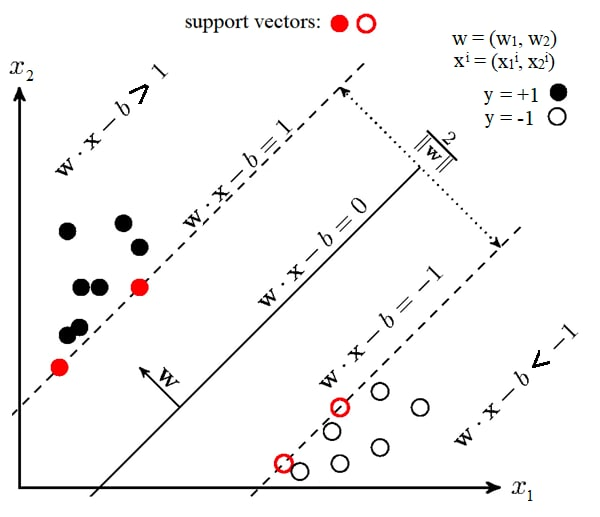
\includegraphics[scale=0.35]{1.jpg}}
\end{figure}

Тогда задачу можно свести к задаче квадратичного программирования с линейными ограничениями:
	$$
	\begin{cases}
		\frac{1}{2}\langle\boldsymbol{w},\boldsymbol{w}\rangle\rightarrow \min\limits_{\boldsymbol{w} }\\
		\left(\langle\boldsymbol{x}_i,\boldsymbol{w}\rangle - w_0\right)y_i \geq 1 \\
	\end{cases}
	$$
 Воспользуемся методом множителей Лагранжа:
	$$
	\begin{cases}
		\inf\limits_{\boldsymbol{w},w_0} \frac{1}{2}\langle\boldsymbol{w},\boldsymbol{w}\rangle - \sum\limits_{i=1}^n\alpha_i\left[y_i\left(\boldsymbol{x}_i^\intercal\boldsymbol{w} + w_0\right)-1\right] \rightarrow \max\limits_{\alpha_i} \\
		\alpha_i \geq 0, \forall i \\
		y_i\left(\large\boldsymbol{x}_i,\boldsymbol{w}\rangle - w_0\right) \geq 1 \\
	\end{cases}
	$$

 Так как оптимизируемая функция гладкая, можно воспользоваться необходимыми условиями экстремума
$$
\frac{\partial}{\partial \boldsymbol{w}}: \boldsymbol{w} = \sum\limits_{i=1}^{n}\alpha_i y_i \boldsymbol{x}_i $$$$
\frac{\partial}{\partial w_0}: 0=\sum\limits_{i=1}^{n}\alpha_i y_i $$
Двойственная задача Вольфа:
$$
	\begin{cases}
		\sum\limits_{i=1}^n \alpha_i - \frac{1}{2}\sum\limits_{i=1}^n\sum\limits_{j=1}^{n}\alpha_i\alpha_jy_iy_j\boldsymbol{x}_i^{T} \boldsymbol{x}_j \rightarrow \max\limits_{\alpha_i} \\
		\alpha_i \geq 0, \forall i \\
		y_i\left(\langle\boldsymbol{x}_i,\boldsymbol{w}\rangle - w_0\right) \geq 1 \\
	\boldsymbol{w}_0 = \sum\limits_{i=1}^{n}\alpha_i y_i \boldsymbol{x}_i \\
 	\end{cases}
$$



    
	В точке оптимума выполнены условия Каруша-Куна-Такера, в частности:
	$$ \alpha_i \left[1-y_i\left(\langle\boldsymbol{x}_i,\boldsymbol{w}\rangle - w_0\right)\right] = 0\, \forall i$$

	Т.е. либо
	\begin{itemize}
		\item $\alpha_i=0$  т.е. наблюдение не влияет на $\boldsymbol{w},w_0$
		\item $\alpha_i>0 \Rightarrow y_i \left(\langle\boldsymbol{x}_i,\boldsymbol{w}\rangle - w_0\right) = 1$ -- такое наблюдение будем называть опорным вектором
	\end{itemize}
	
	
\subsection{SVM.Slack variables}
	Поскольку в случае линейно неразделимой выборки по определению любой линейный классификатор будет
ошибаться, условие $\left(\langle\boldsymbol{x}_i,\boldsymbol{w}\rangle - w_0\right)y_i \geq 1$ не может быть выполнено для всех $i$. Введём ошибки $\xi \geq 0$ алгоритма и штрафы за эти ошибки в минимизируемую функцию следующим образом:
$$
	\begin{cases}
		\frac{1}{2}\langle\boldsymbol{w},\boldsymbol{w}\rangle+C\sum\limits_{i=1}^n\xi_i\rightarrow \min\limits_{\boldsymbol{w},w_0 }\\
		\left(\langle\boldsymbol{x}_i,\boldsymbol{w}\rangle - w_0\right)y_i \geq 1 -\xi_i\\,
	\end{cases}$$
где C задает размер штрафа за ошибки.

Мы опять получили задачу линейного программирования.
\begin{figure}[h!]
\center{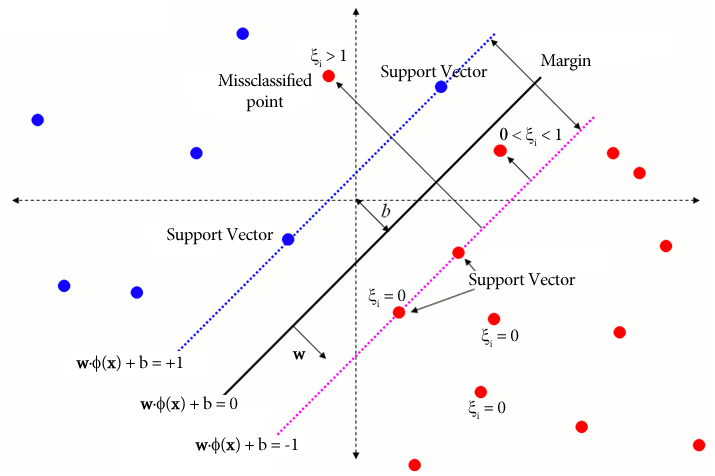
\includegraphics[scale=0.45]{2.png}}
\end{figure}


\subsection{Kernel trick} 
Чтобы применять SVN в нелинейном случае, строилось спрямляющее пространство. В основе этого лежит
очень простая и очень красивая идея: если в каком-то исходном пространстве признаков классы не являются
линейно разделимыми, то может быть можно отобразить это пространство признаков в какое-то новое, в
котором классы уже будут линейно разделимы.

Пусть $\phi (\boldsymbol{x}_i)$ - спрямляющее отображение. Тогда, можем записать SVM в спрямляющем отображении, используя следующее скалярное произведение:
$$ \boldsymbol{x}_i \rightarrow \phi (\boldsymbol{x}), ~ \boldsymbol{w} \rightarrow \phi (\boldsymbol{w}), ~ \langle \boldsymbol{w}, \boldsymbol{x}_i \rangle \rightarrow \langle  \phi (\boldsymbol{w}), \phi (\boldsymbol{x}_i) \rangle$$

Чтобы получить нелинейную разделимость в исходном пространстве - зададим скалярное произведение следующего вида:
$$K(\boldsymbol{w}, \boldsymbol{x}_i) = \langle  \phi (\boldsymbol{w}), \phi (\boldsymbol{x}_i) \rangle$$
$K$ - симметричная нелинейная функция



\begin{figure}[h!]
\center{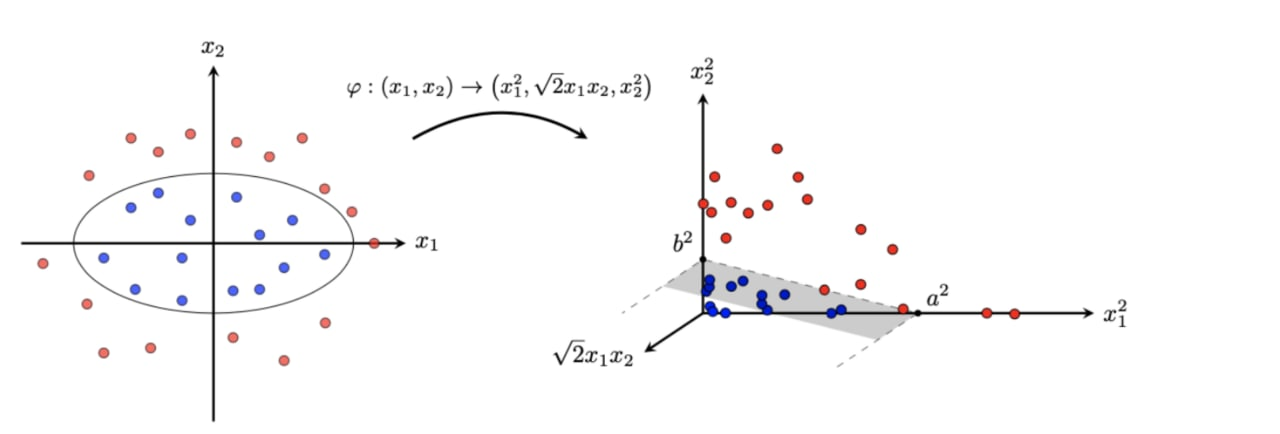
\includegraphics[scale=0.27]{5.jpg}}
\end{figure}


Наиболее часто используемые ядра
\begin{itemize}
\item Линейное ядро:
$$K(\boldsymbol{w}, \boldsymbol{x}_i) = \langle \boldsymbol{w}, \boldsymbol{x}_i \rangle$$

\item Полиномиальное ядро:
$$K(\boldsymbol{w}, \boldsymbol{x}_i) = (\langle \boldsymbol{w}, \boldsymbol{x}_i \rangle + r)^d$$

\item Радиальное ядро:
$$K(\boldsymbol{w}, \boldsymbol{x}_i) = exp(-\gamma ||(\boldsymbol{w}-\boldsymbol{x}_i)||^2)$$
\item Сигмовидное ядро.
\end{itemize}
Примеры:

\begin{figure}[h!]
\center{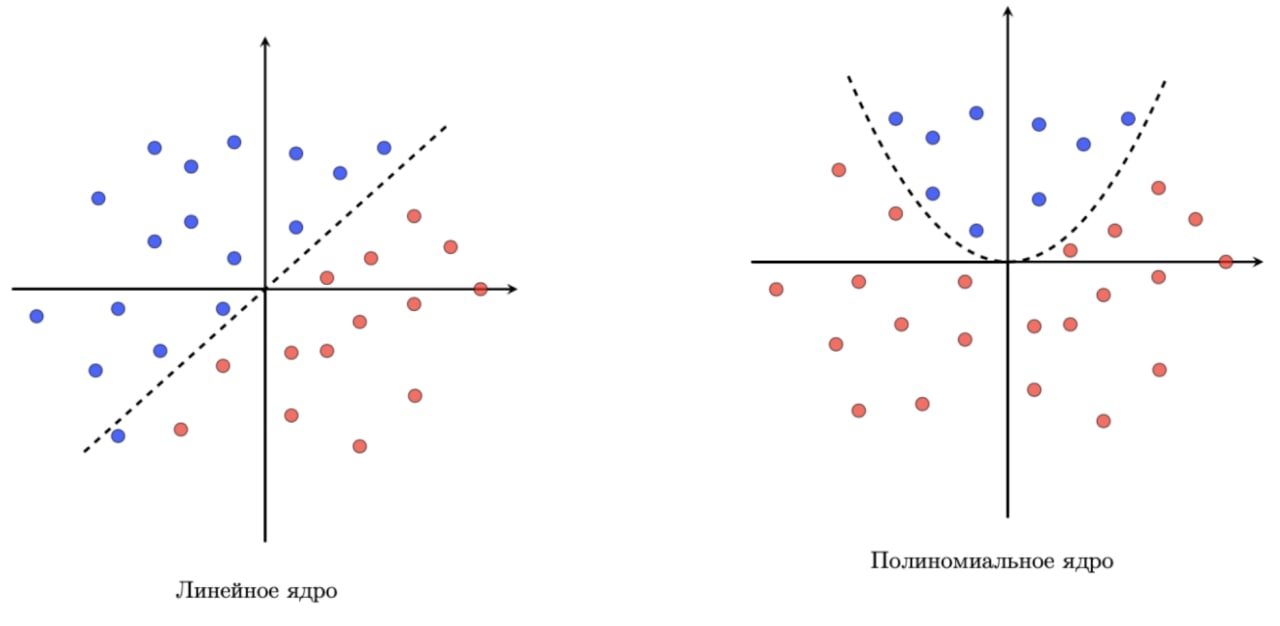
\includegraphics[scale=0.25]{3.jpg}}
\end{figure}
\begin{figure}[h!]
\center{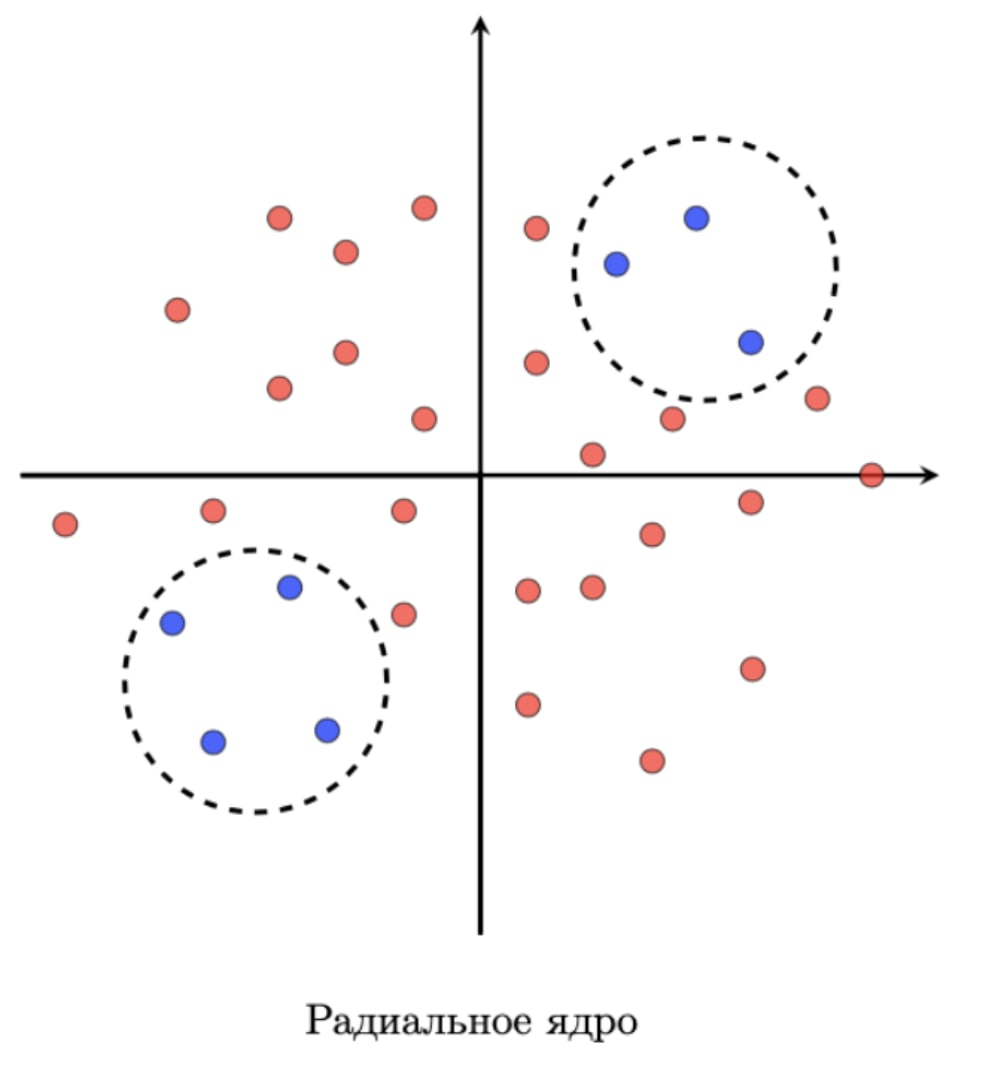
\includegraphics[scale=0.10]{4.jpg}}
\end{figure}
\begin{figure}[h!!]
\center{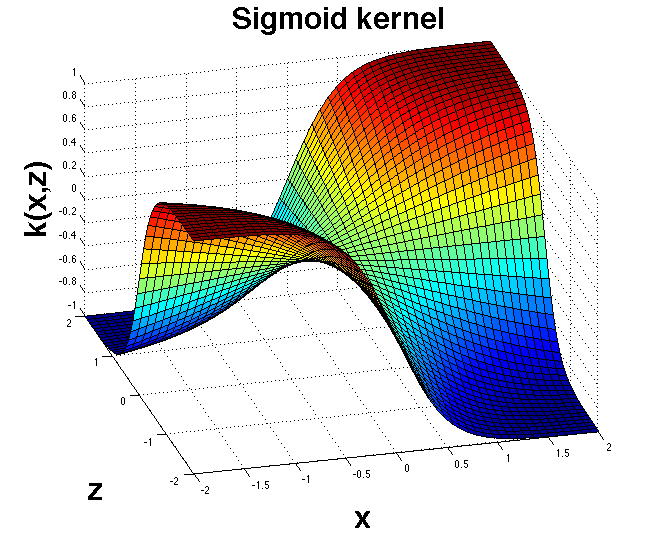
\includegraphics[scale=1]{sigm.png}}
\caption{Сигмовидное ядро}
\end{figure}

\subsection{Сложность SVM} 
Так как для SVM нужно решать задачу квадратичного программирования, то сложность варьируется между $O(p\cdot n^2)$ и $O(p\cdot n^3)$, где $p$ -- количество признаков, $n$ -- количество индивидов, зависимости от набора данных. 
\subsection{Мультиклассовый SVM} 

\begin{itemize}
    \item Сравнение "один со многими". 
 Строим $N$ классифицирущих правил $f_i(\boldsymbol{x})$, кодирующих принадлежность к $i$-му классу за 1, -1 иначе. В качестве решающего правила используется
    $$f(\boldsymbol{x}) = \underset{i}{argmax} f_i(\boldsymbol{x})$$ 

\item Сравнение "каждый с каждым". 
Строим $\frac{N(N-1)}{2}$ классифицирущих правил, производящих классификацию для каждой возможной пары классов. Обозначим за $N_i$ количество сравнений, в которых элемент $x$ был классифицирован как принадлежный к $i$-му классу. В качестве решающего правила используется
    $$f(\boldsymbol{x}) = \underset{i}{argmax} N_i$$ 

\end{itemize}

\section{Логистическая регрессия}
\subsection{Логистическая регрессия. Подход через минимизацию функции потерь}
Линейная модель классификации: 
\begin{itemize}
	\item $f(x, \theta)=\sign \langle \theta,x\rangle,~~ x,\theta\in \mathbb{R}^p$
	\item $M=\langle \theta,x \rangle y$ --- отступ.
\end{itemize}

В качестве аппроксимации пороговой функции потерь берется логарифмическая функция потерь $L(M)=\log(1+e^{-M}).$

\begin{figure}[hhh!]
	\begin{center}
		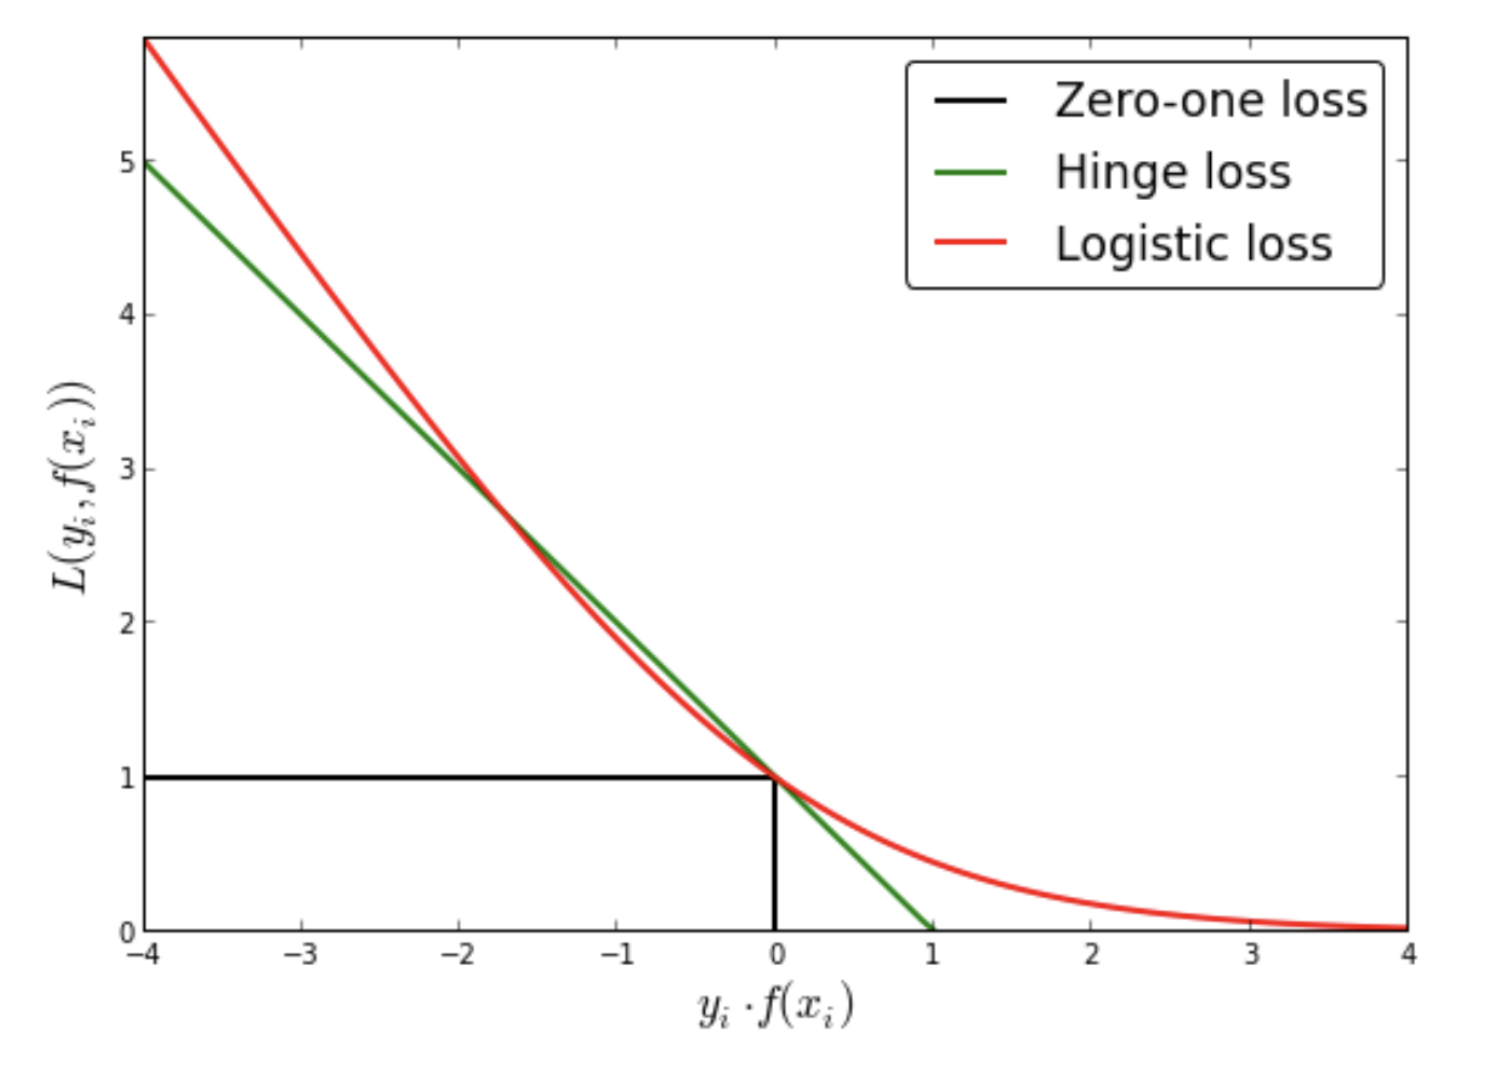
\includegraphics[width=10cm]{loss_function}
	\end{center}
	\vspace{-5mm}
\end{figure}

\newpage

\begin{task}
	$\mathsf{Q(X_n, \theta)=\sum \limits_{i=1}^n \log (1+\exp{(-y_i\langle \theta,x_i\rangle)}) \to \min \limits_{\theta}}$
\end{task}
Методы решения задачи минимизации:
\begin{itemize}
	\item метод стохастического градиента
	\item метод Ньютона-Рафсона
\end{itemize}


\subsection{Логистическая регрессия. Вероятностный подход}
$\mathsf{P(y = 1|x,\theta)=\sigma_\theta(M)=\frac{1}{1+e^{-\langle x,\theta \rangle y}}}$ --- сигмоидная функция. \\
Свойства $\mathsf{\sigma(z)}$:

\begin{itemize}
	\item $\mathsf{\sigma(z)} \in [0,1]$ , задана на $(-\infty,+\infty)$
	\item {$\mathsf{\sigma(z)\to 1,~ z\to +\infty};$ $\mathsf{\sigma(z)\to 0,~ z\to -\infty} $}
	\item $\mathsf{\sigma(z)+\sigma(-z)=1}$
	\item $\mathsf{\sigma ' (z)=\sigma (z)\sigma(-z)}$
\end{itemize}

\begin{figure}[h!]
	\begin{center}
		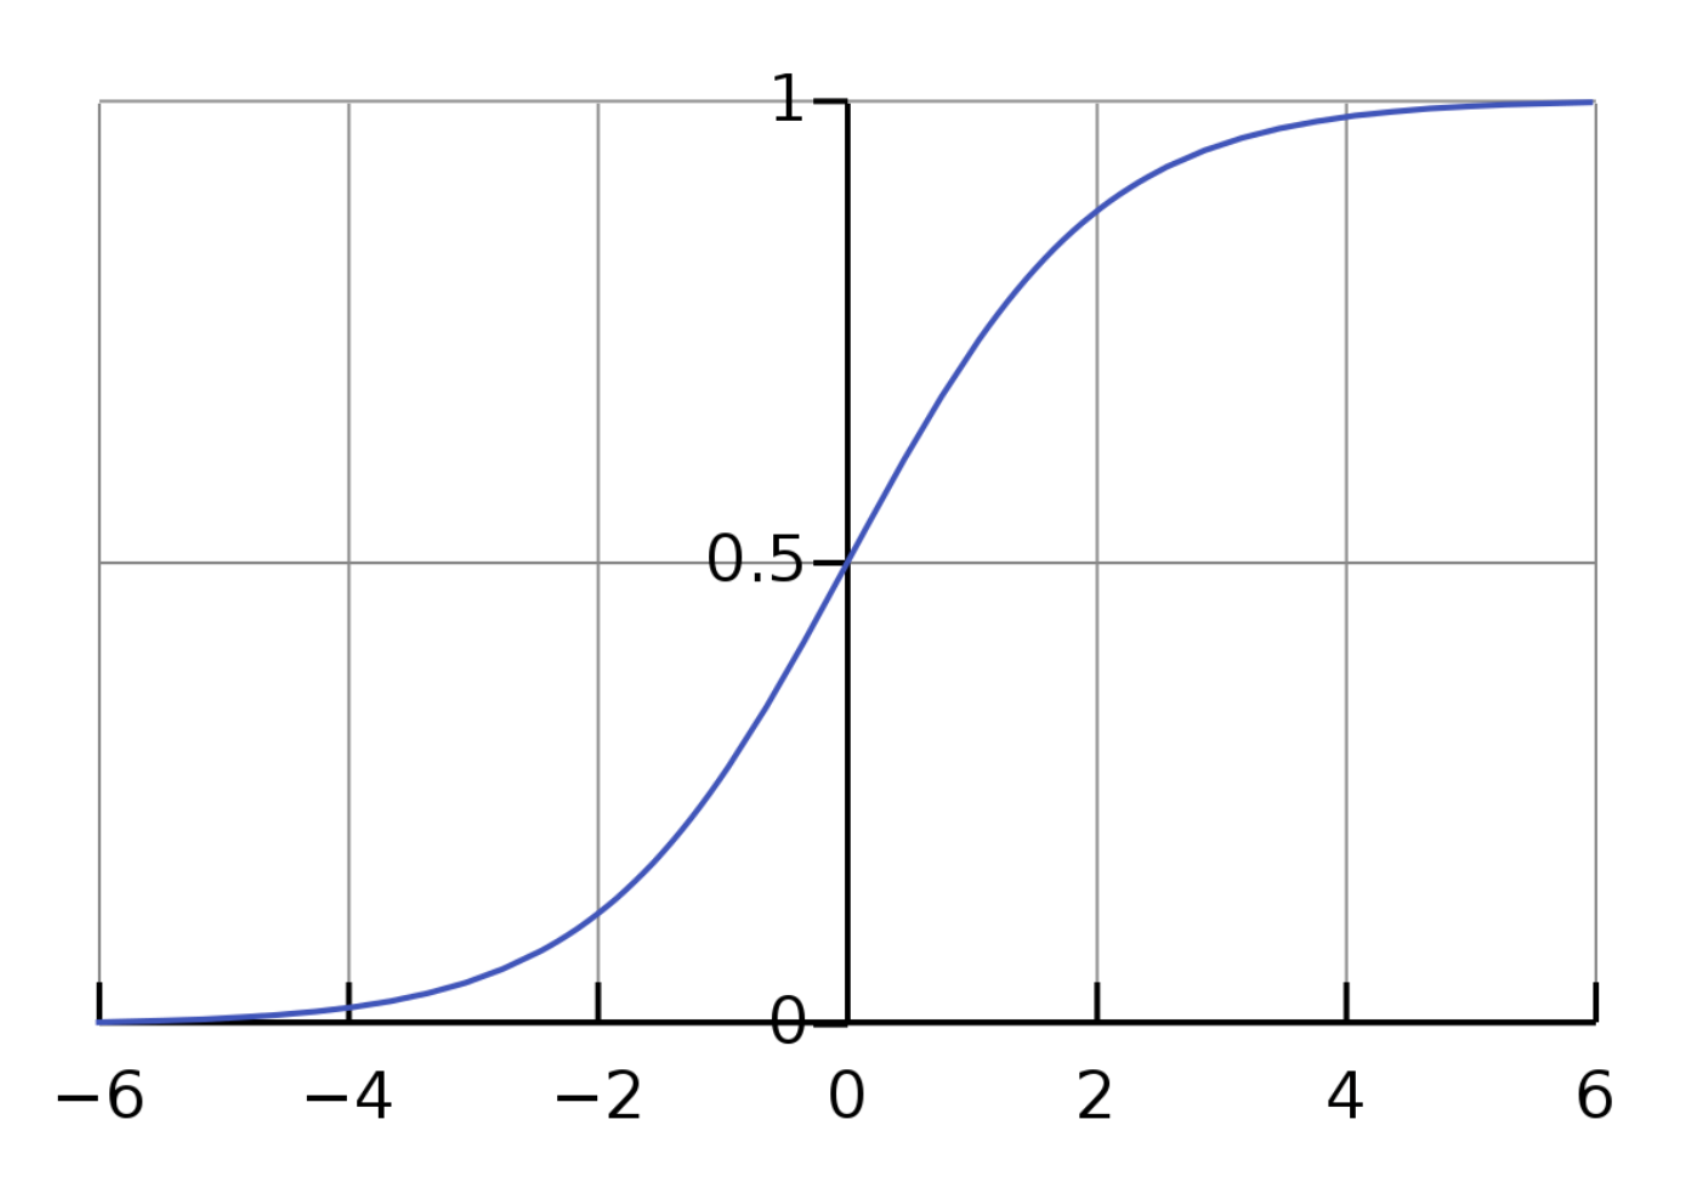
\includegraphics[width=10cm]{sigmoid2}
	\end{center}
	\caption{Сигмоидная функция}
	\vspace{-5mm}
\end{figure}

\newpage

Пусть $\mathsf{Y}=\{0,1\}$.
\begin{itemize}
	\item $\mathsf{P(y_i=1|x;\theta)=\sigma_\theta(x)}$
	\item $\mathsf{P(y_i=0|x;\theta)=1-\sigma_\theta(x)}$
\end{itemize}
Тогда $\mathsf{P(y|x;\theta)=(\sigma_\theta(x))^y(1-\sigma_\theta(x))^{1-y}}.$ \\
Функция правдоподобия:
\begin{equation*}
	\mathsf{Q(X_n, \theta)=-\log L(\theta)=-\log \prod\limits_{i=1}^n(\sigma_\theta(x_i))^{y_i}(1-\sigma_\theta(x_i))^{1-y_i}}= 
\end{equation*}
\begin{equation*}
	=\mathsf{-\sum\limits_{i=1}^n [y_i\log (\sigma_\theta(x_i)+(1-y_i))\log (1-\sigma_\theta(x_i))]\to \min\limits_{\theta}}
\end{equation*}

\subsection{Линейная и логистическая регрессия}

Существуют примеры данных, для которых логистическая регрессия показывает лучшие результаты, чем линейная.

\begin{figure}[h!]
	\begin{center}
		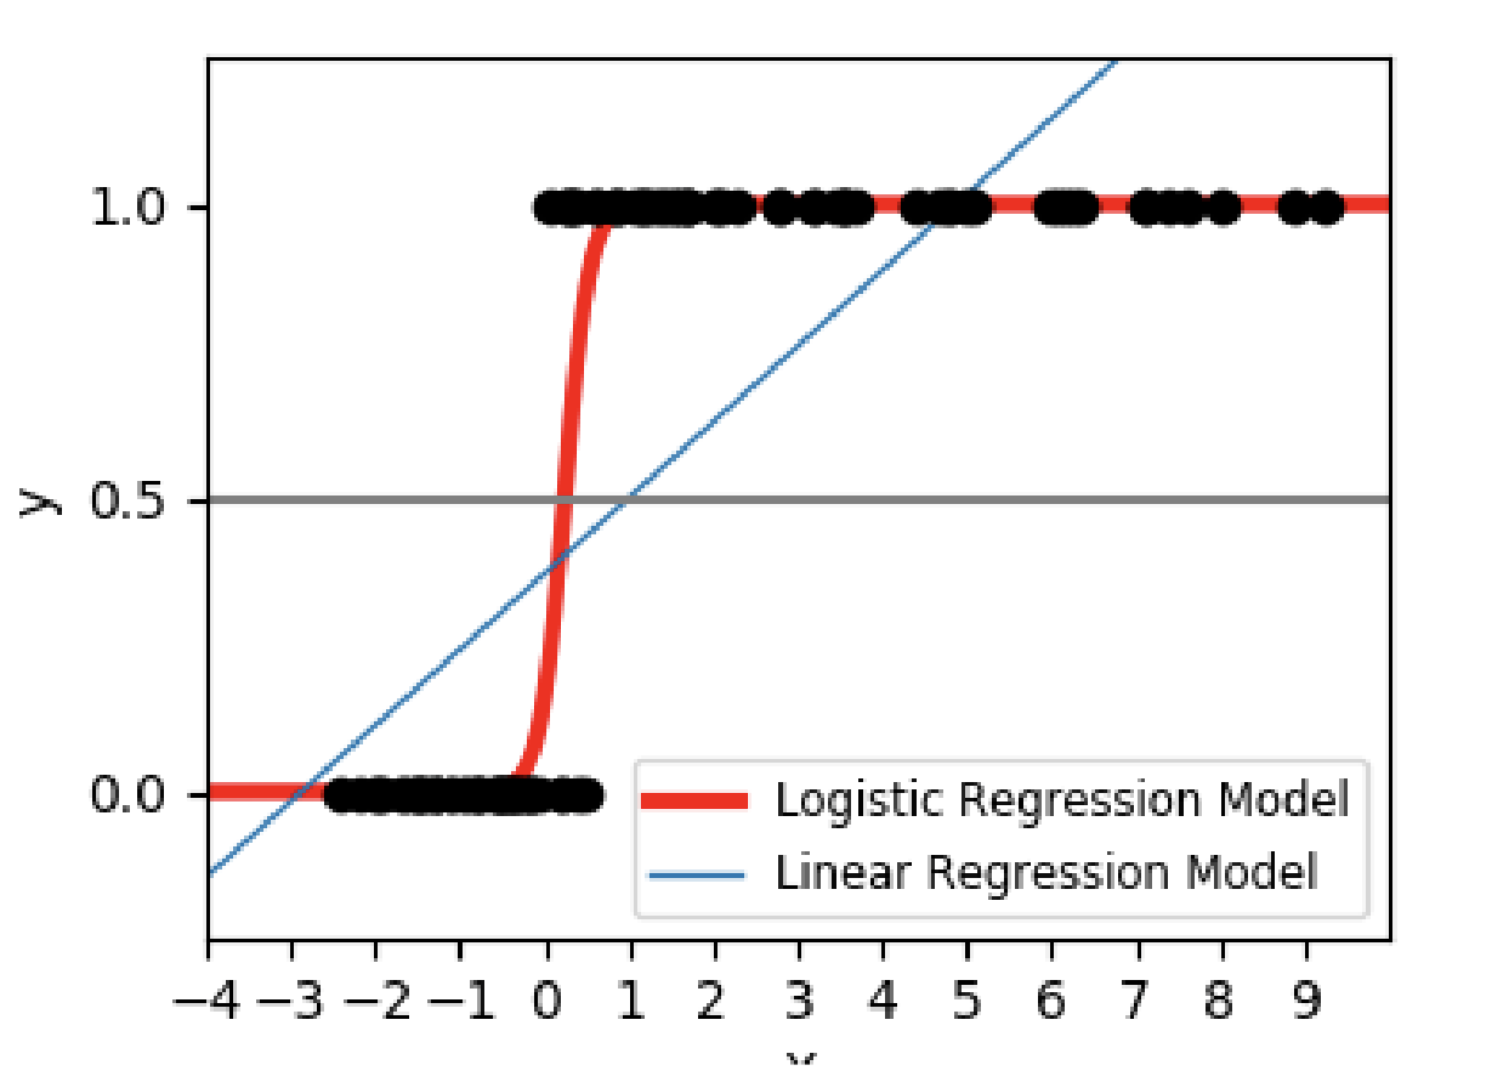
\includegraphics[width=10cm]{regression}
	\end{center}
	\caption{Линейная и логистическая регрессия}
	\vspace{-5mm}
\end{figure}

\subsection{Логистическая регрессия. Регуляризация}
$\mathsf{Q(\theta)=-\sum\limits_{i=1}^n [y_i\log (\sigma_\theta(x_i)+(1-y_i))\log (1-\sigma_\theta(x_i))]}$

Регуляризация в логистической регрессии:
\begin{itemize}
	\item {{\bf L2}: 
		$\mathsf{Q_\tau(\theta)=Q(\theta)+\frac{\tau}{2}\sum\limits_{j=1}^p \theta_j^2 \to \min\limits_\theta}$
	}
	\item {{\bf L1}: 
		$\mathsf{Q_\tau(\theta)=Q(\theta)+\tau\sum\limits_{j=1}^p |\theta_j| \to \min\limits_\theta}$
	}
\end{itemize}
Параметр $\mathsf{\tau}$ можно подбирать с помощью кросс-валидации. \\
Методы решения задачи минимизации: 
\begin{itemize}
	\item метод стохастического градиента
	\item метод Ньютона-Рафсона.
\end{itemize}

\subsection{Многоклассовая логистическая регрессия}
Линейный классификатор при произвольном числе классов $\mathsf{Y=\{1,\ldots,K\}}$: 
\begin{equation*}
	\hat{f}(x,\theta)=\argmax_{y\in Y}\langle \theta_y,x \rangle, \ x,\theta_y\in\mathbb{R}^p
\end{equation*}
Вероятность того, что объект $x$ относится к классу $i$:
\begin{equation*}
	\mathsf{P}(y=i|x;\theta)=\frac{\exp{\langle \theta_y,x \rangle}}{\sum\limits_{z\in Y}\exp{\langle \theta_z,x \rangle}}=\frac{e^{\theta_i^{\mathrm{T}}x}}{\sum\limits_{k=1}^Ke^{\theta_k^{\mathrm{T}}x}}
\end{equation*}
Задача:
\begin{equation*}
	\mathsf{Q(X_n, \theta)=-\sum\limits_{i=1}^n\log P(y_i|x_i;\theta)\to \min\limits_\theta }
\end{equation*}

\subsection{Логистическая регрессия. Преимущества и недостатки}
Плюсы:
\begin{enumerate}
	\item Позволяет оценить вероятности принадлежности объектов к классу
	\item Достаточно быстро работает при больших объемах выборки
	\item Применима в случае отсутствия линейной разделимости, если на вход подать полиномиальные признаки
\end{enumerate}
Минусы:
\begin{enumerate}
	\item Плохо работает в задачах, в которых зависимость сложная, нелинейная
\end{enumerate}

\end{document}